\begin{frame}{Ice People Family Tree}
    \note{\tiny
    \begin{itemize}

        \item Diving into the narrative intricacies of the 47-book saga,
        we're brought face-to-face with a sprawling family tree that traces its lineage
        back to the matriarch Silja Arngrímsdóttir and her cursed beau, Þengill the good.

        \item Their descendants' tangled relationships are laid out here,
        and it's impossible to ignore the density of the connections --
        hinting at a significant amount of inbreeding.
        This compact lineage, while perhaps challenging for readers (and narrators!)
        to digest given its incestuous undertones, does offer us a silver lining --
        it's surprisingly \emph{slide-friendly}. Managing to represent 17 generations in one visual
        would generally be a challenge, but the Ice People's family tree is a rare exception.

        \item On the topic of the curse, those afflicted by it have been highlighted with solid colors.
        The color codes represent their nature: yellow for the \emph{virtuous},
        green for the \emph{malevolent}, and pink for those who found \emph{redemption},
        transitioning from darkness to light.

        \item As we scan through the tree, it's curious to note that the distribution of the curse
        doesn't seem to follow a strict genetic pattern. Entire generations sometimes escape its grasp,
        suggesting that Margit perhaps allowed a degree of creative freedom over genetic accuracy in
        deciding who bears the curse.

        \item This intricate web of relationships, filled with cursed figures,
        highlights the need for a data-driven approach to unravel and understand Margit's artistic choices.
        \end{itemize}
}
    \centering
    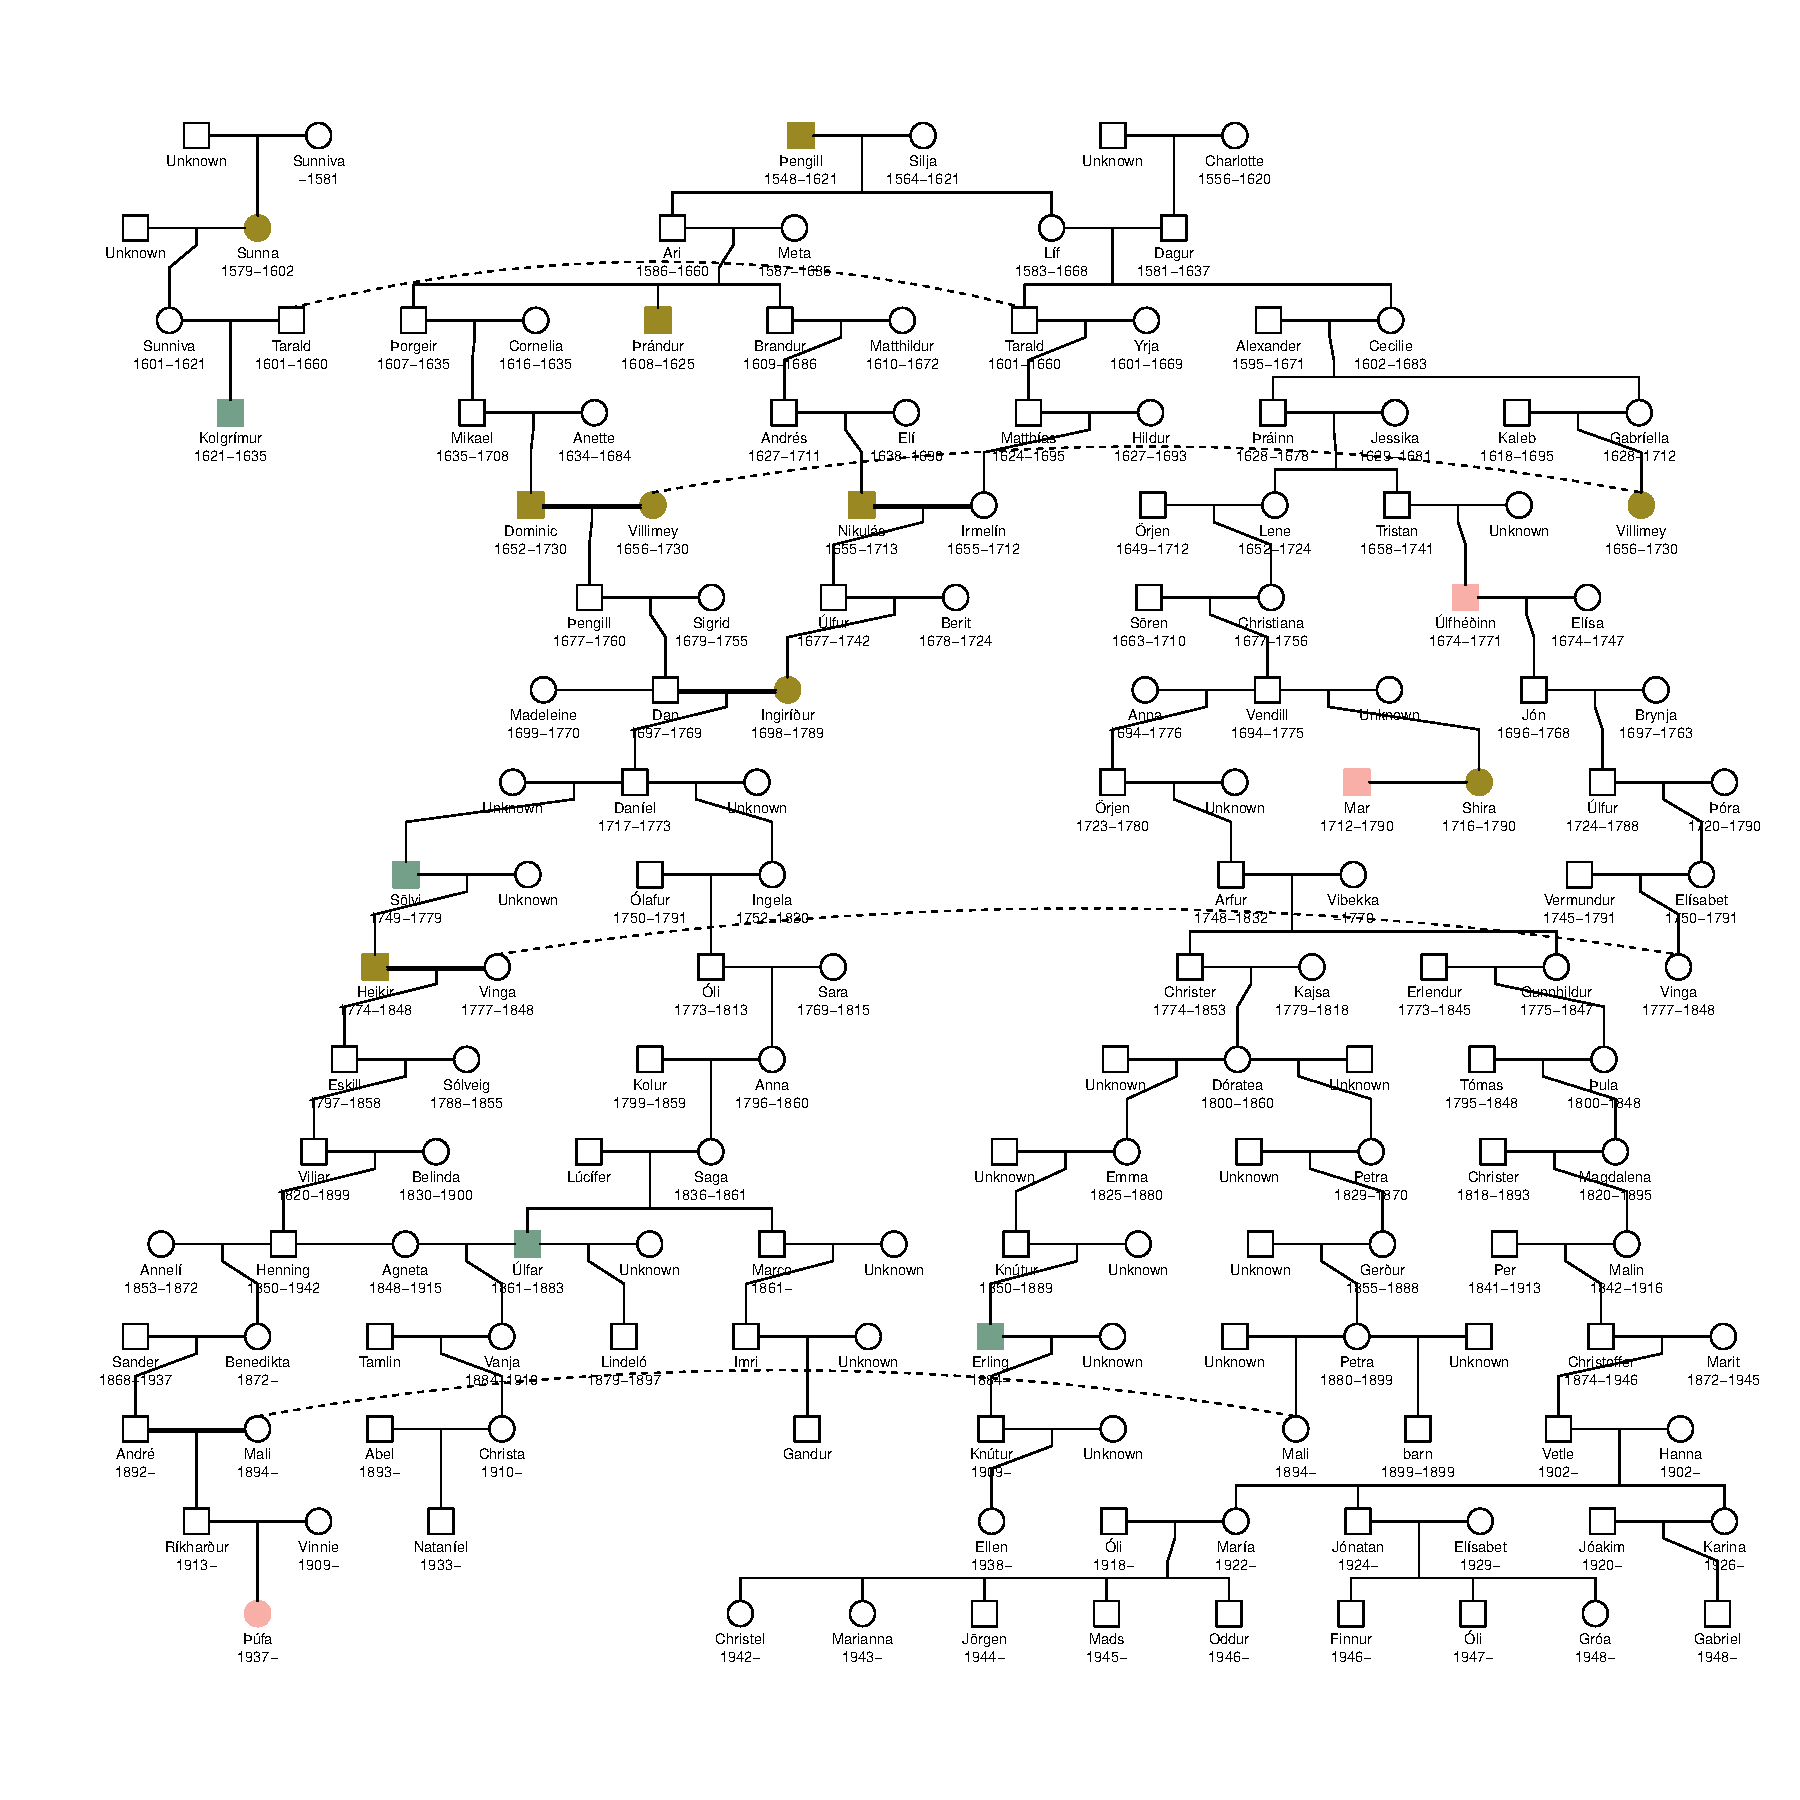
\includegraphics[height=.9\textheight]{../rek-data-beers/R/figures/family_tree}
\end{frame}

\begin{frame}{Ice People Family Gantt Chart}
    \note{\tiny
    \begin{itemize}
        \item To decipher the complex family tree and its concurrent relationships,
        we turned to a \emph{data transformation}: the \emph{Gantt} chart,
        usually a tool for project timelines, but here, it's a brilliant
        visualization of lifespans and intersecting narratives.

        \item As we traverse this visual representation, you'll notice each individual's
        lifespan is represented by a horizontal bar.
        Births commence on the left and deaths conclude on the right.
        Our familiar color-coding prevails: yellow signifies the benevolent,
        green the malevolent, and pink the redeemed.

        \item Spanning from the mid-1600s to the 1960s, this chart offers clear insights
        into overlapping lifetimes, painting a vivid picture of contemporaneous
        characters.

        \item A pattern quickly emerges: Margit frequently intertwines character narratives,
        often through romantic unions. This attraction amongst the Ice People is
        both a narrative device and a manifestation of their shared, cursed lineage.
        While generations pass, the family typically hovers around 20 living members,
        swelling to 30 towards the end.

        \item Worth noting is the general pattern of having 1-2 cursed individuals alive at
        any point. Yet, in the early 1700s, a deviation occurs with six concurrent
        cursed beings. And while Mar doesn't emerge until later in the narrative,
        he isn't directly from the Ice People lineage but descends from the Taranqyes.
        This clan shares a common ancestor with the Ice People, tracing back to
        the malevolent Þengill the Bad.
        \end{itemize}
    }
    \centering
    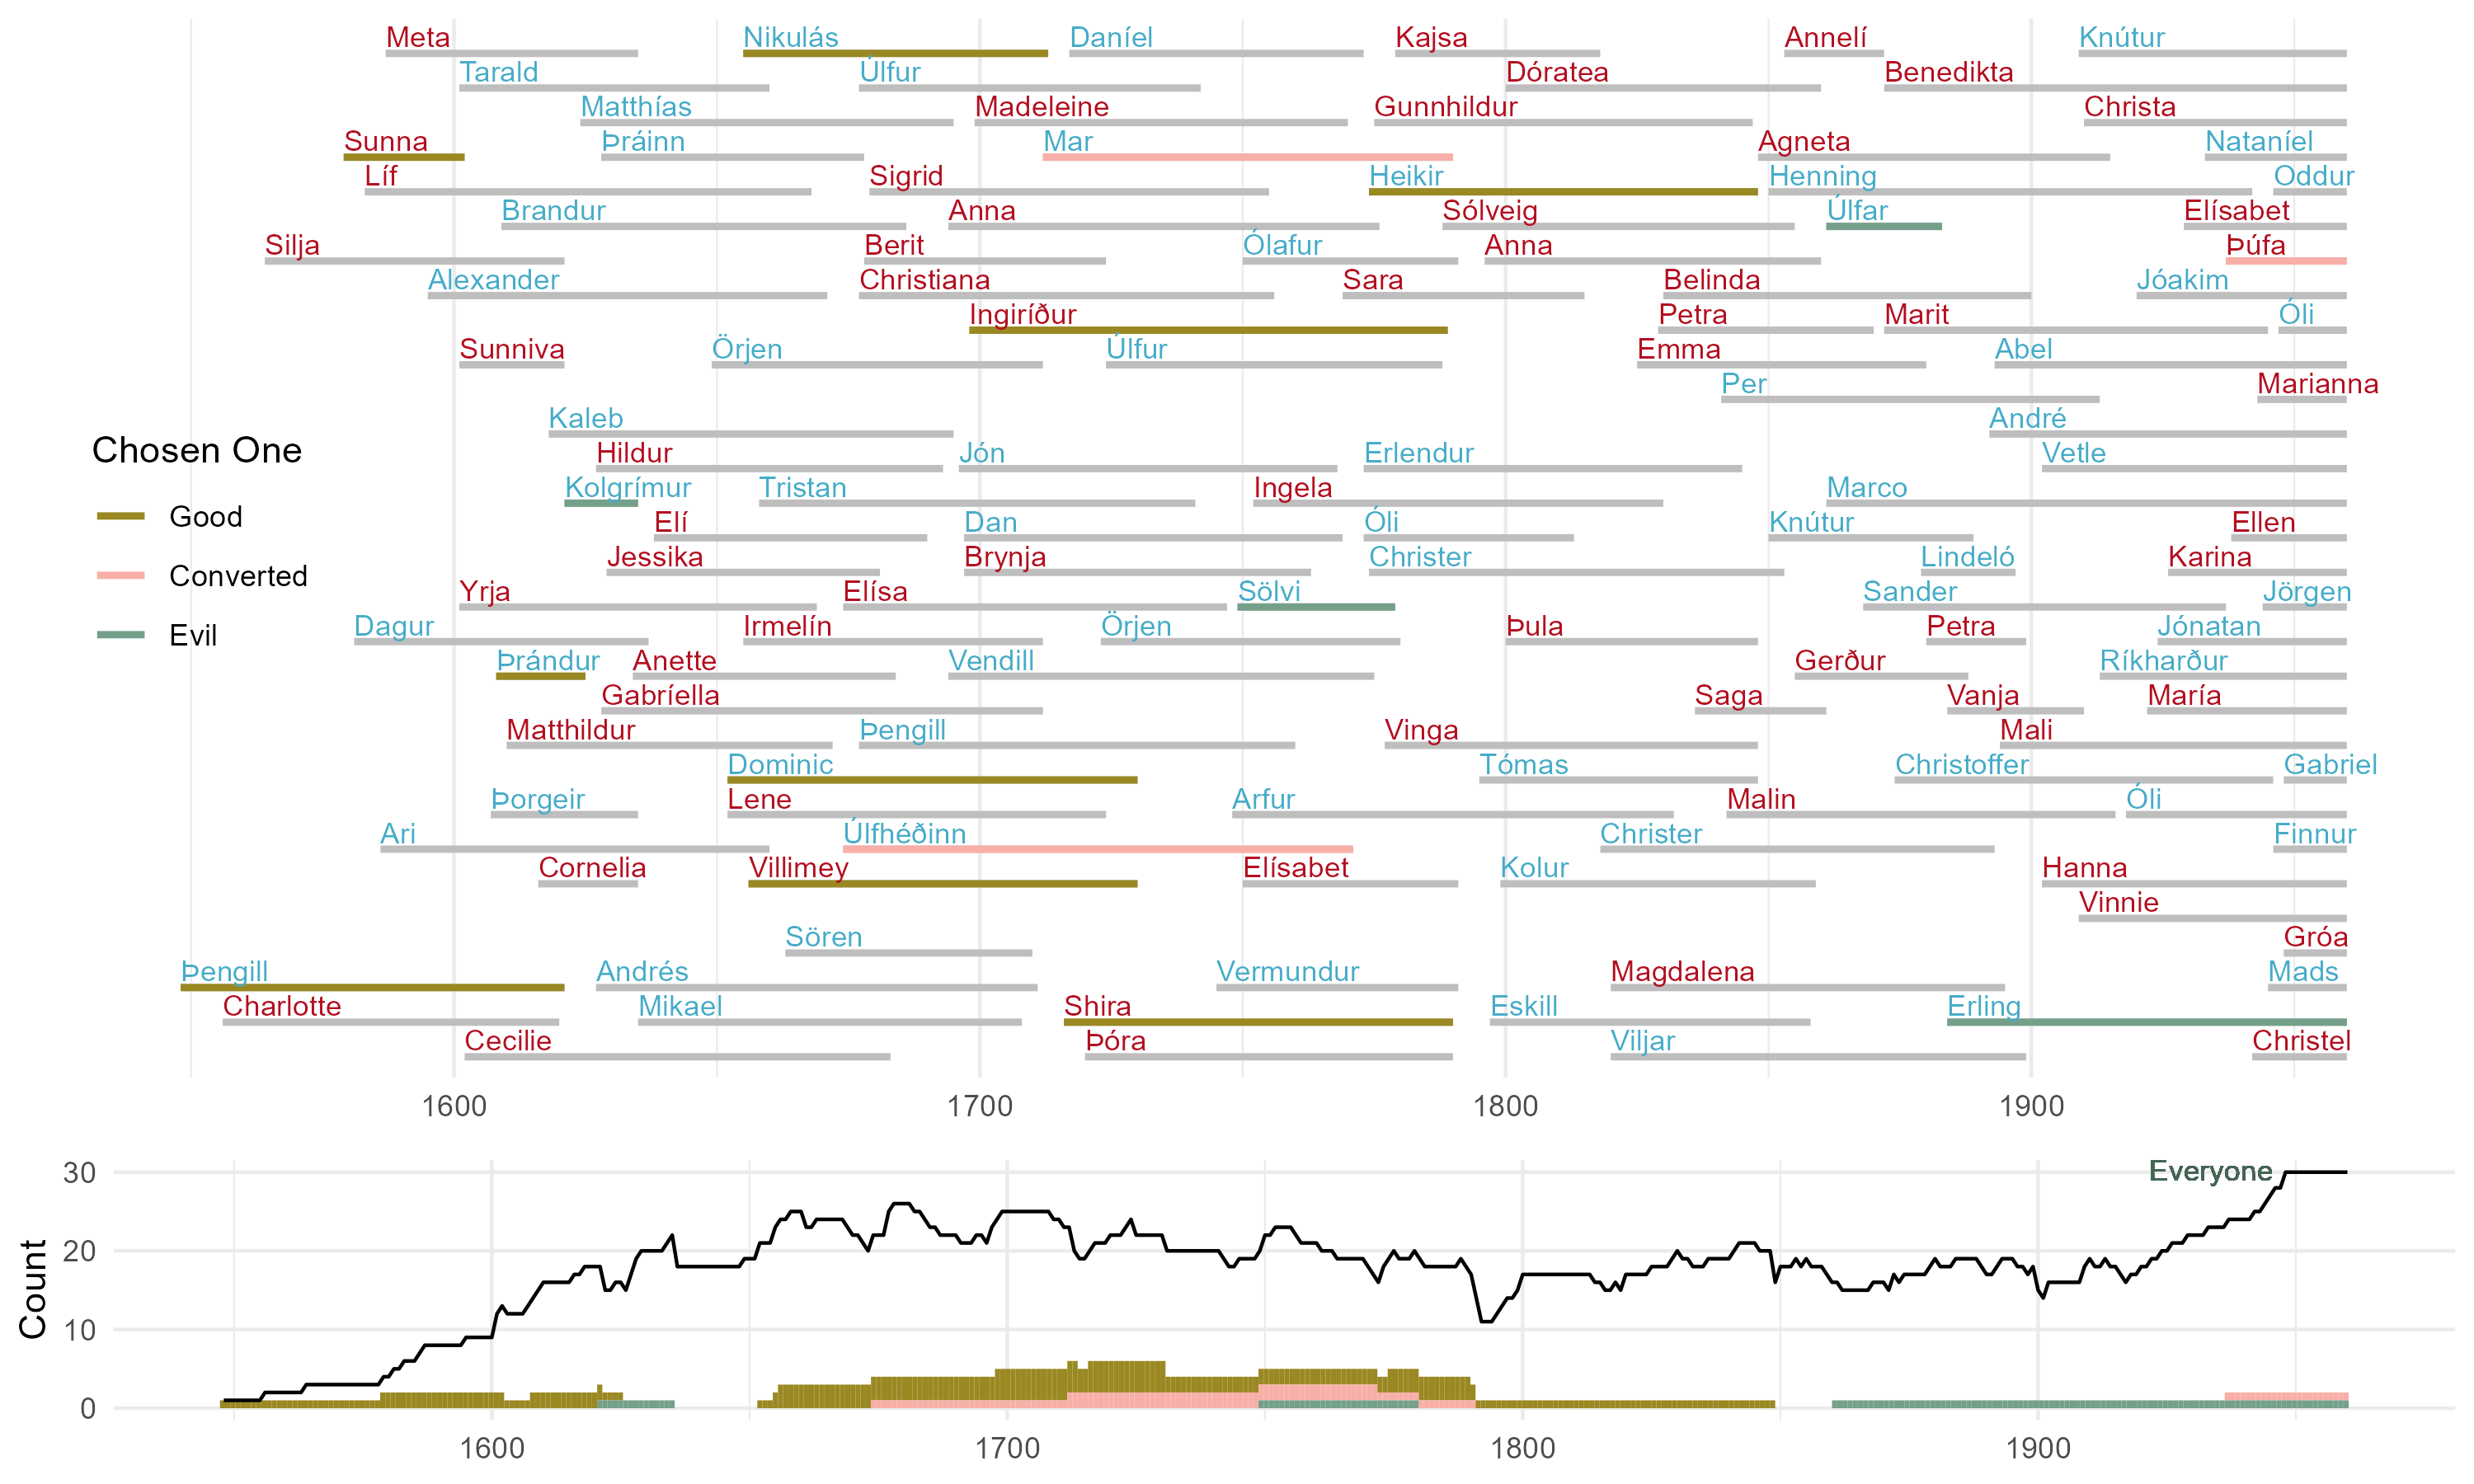
\includegraphics[width=\textwidth]{../rek-data-beers/R/figures/family_gantt}
\end{frame}

\begin{frame}{Lifespan of the Ice People}
\note{\tiny
\begin{itemize}
\item The world of \emph{ÍSFÓLKIÐ} presents a peculiar age distribution.
Unlike the unimodal tendencies we see in the real world, the saga demonstrates a pronounced \emph{bimodal distribution}.

\item Women in this universe are especially vulnerable during childbirth, leading to a considerable dip in life expectancy.
This culminates in the first peak of the distribution, which gravitates around the mid-20s.

\item On the brighter side, women who transcend this peril often find themselves blessed with longevity,
creating a second, older age peak close to 70 years.

\item Margit ensures symmetry in her storytelling. Just as the women face the perils of childbirth,
the men aren't spared either. Defined by their audacity and recklessness,
they too often meet early ends.
But much like their female counterparts, those who evade these early hazards can anticipate extended lifespans,
further reinforcing the saga's bimodal age pattern.

\item Now, something that might not be immediately evident from the family tree, but is quite fascinating, are the relationships within the family.
        \begin{itemize}
        \item Only about a third of the characters are not related to the Ice People lineage,
        or as one might refer to them, \emph{muggles}.
        \item Half of the characters are pure-bloods, meaning both their parents are Ice People.
        \item The remaining 15\% are half-bloods.
        \end{itemize}

\end{itemize}
}

    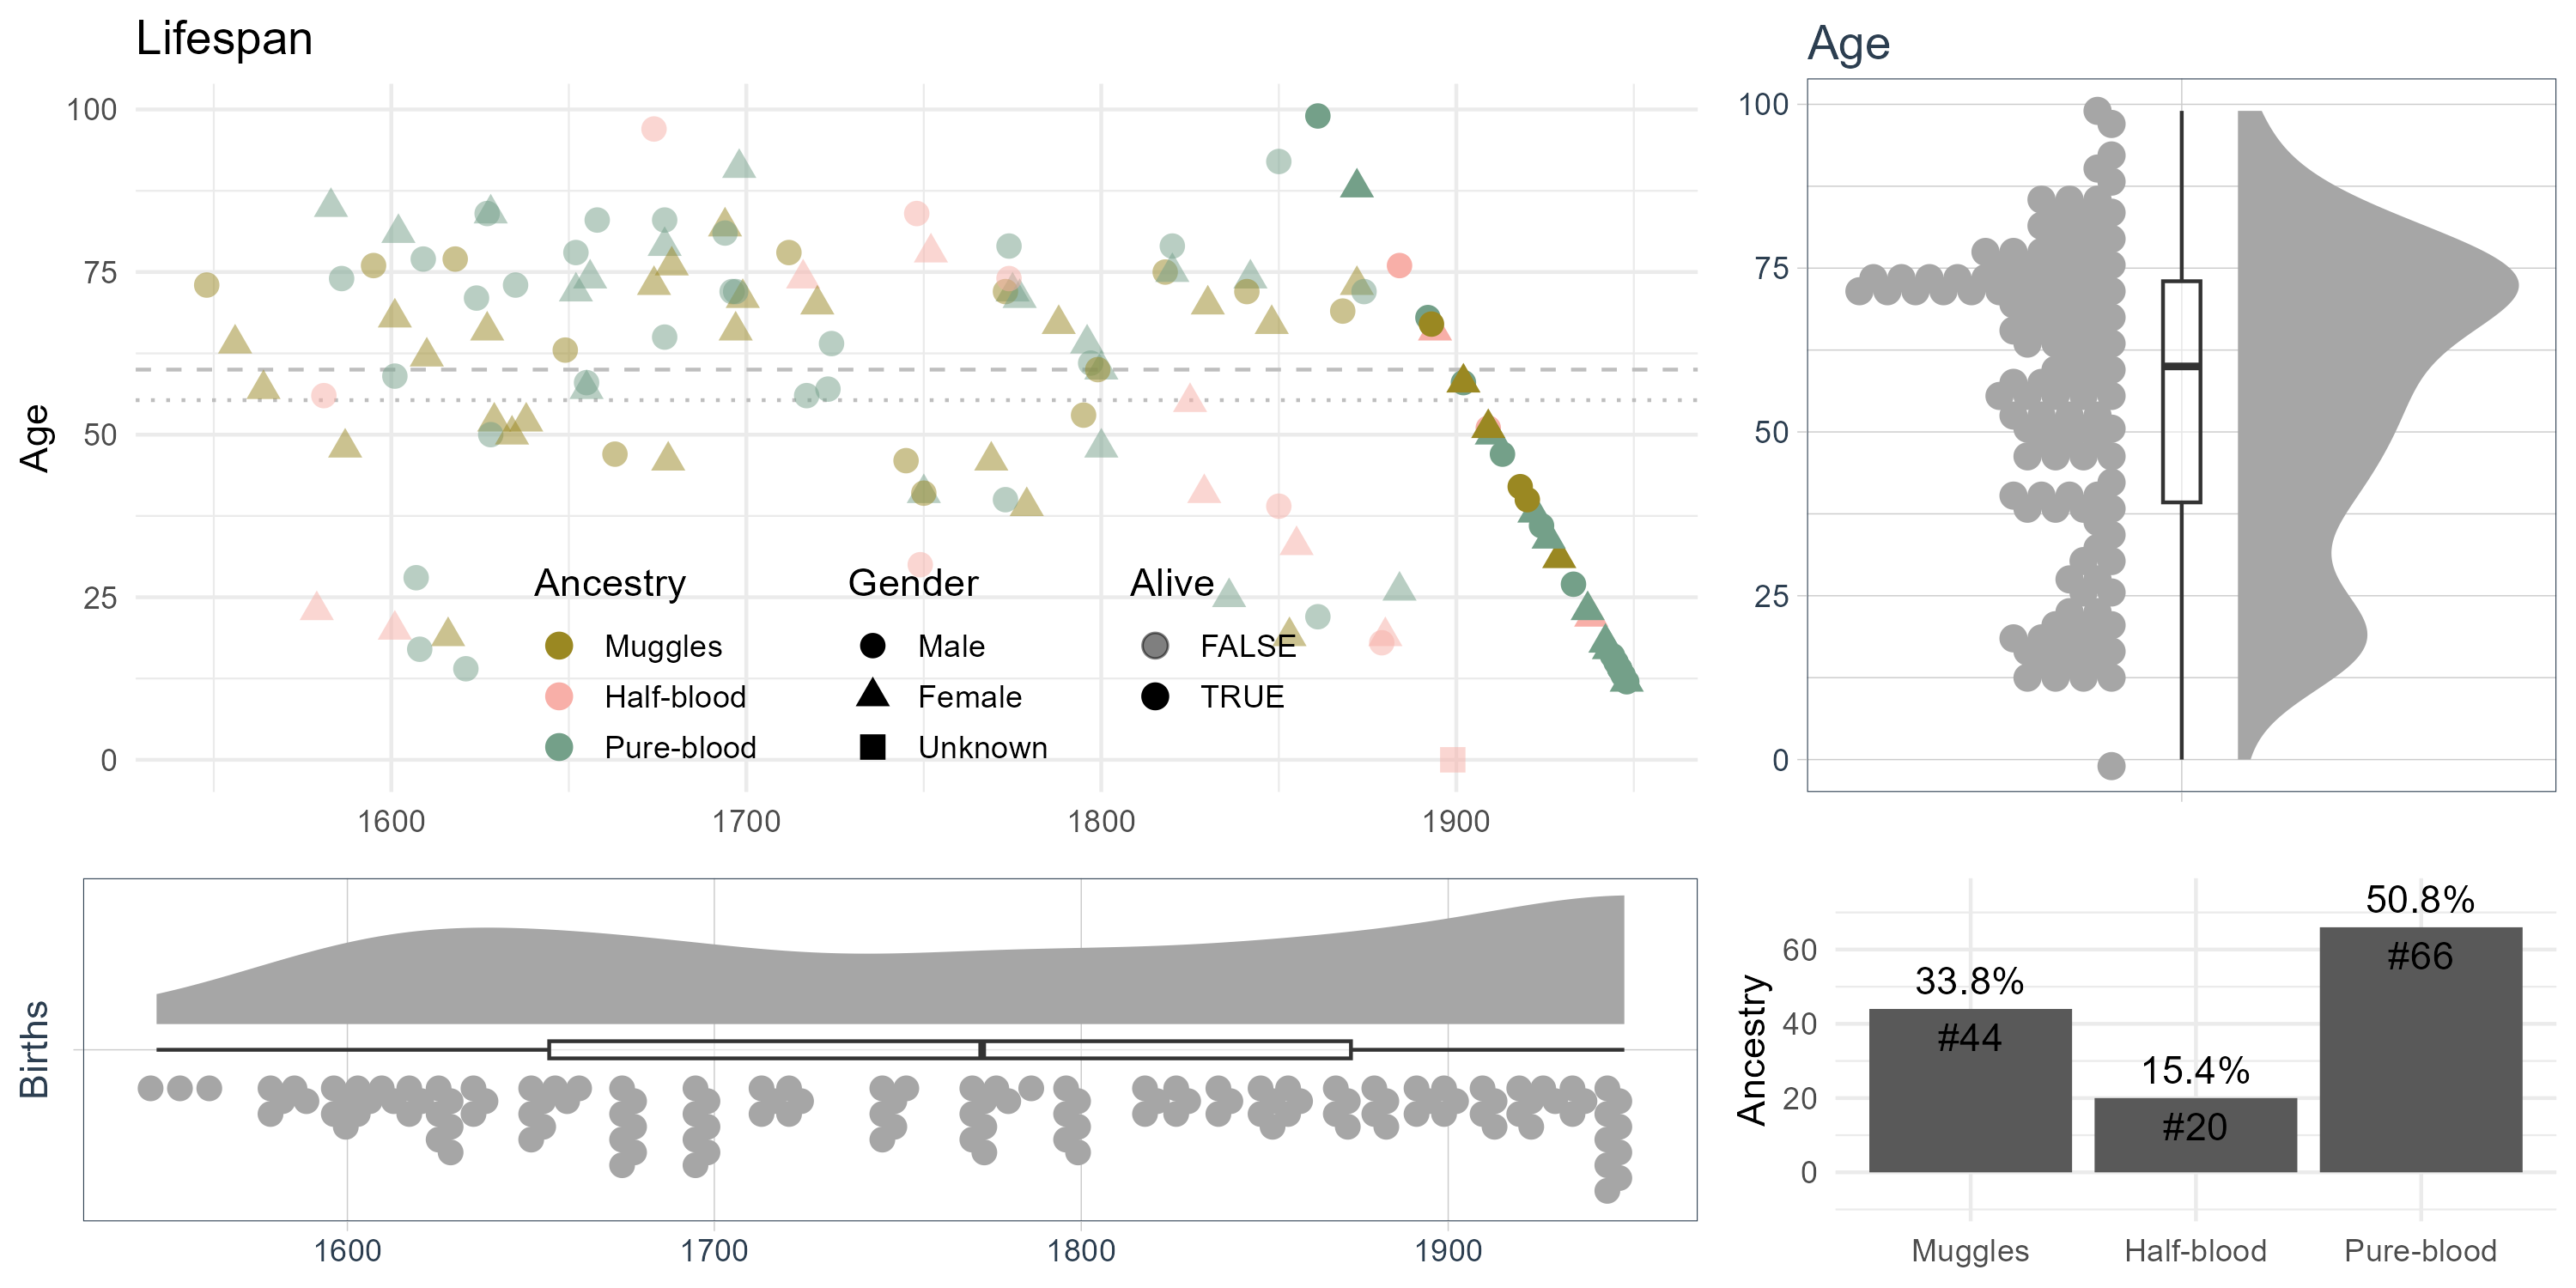
\includegraphics[width=\textwidth]{../rek-data-beers/R/figures/family_birth}
    \vspace{-18pt}
    \begin{itemize}
        \item Average woman lives 58.5 years (median 65, $n=50$)
        \item Average man lives 62.5 years (median 71, $n=49$)
        \item 1 centenarian, 4 people live to 90, 14 live to 80, 46 live to 70
    \end{itemize}
\end{frame}

\begin{frame}{Parental Age Trends \& Marital Age Gaps}
    \note{\scriptsize
      \begin{itemize}
          \item The saga's data reveals that, against the backdrop of potential dangers, women in the Ice People
          generally become mothers at about 23.5 years of age.

          \item Family size decisions are closely tied to the curse. A single non-cursed child often halts further
          family expansion. In contrast, the birth of a cursed child seems to have the opposite effect, leading to larger families,
          under the belief that the generation's \emph{curse quota} has already been met.

          \item A stark reality in the saga is the prevalence of parental absence: one-third of the children grow up
          without one or both parents. Not a mystical cause, but often the stark reality of abandonment.

          \item Yet, amidst these peculiarities, some aspects mirror our world. In 85\% of Ice People marriages,
          husbands are typically older by an average of three years — a trend not uncommon in our own society.
        \end{itemize}
    Delving into the Ice People's world, we find a balance of familiar patterns interwoven with the saga's unique, extraordinary elements.
    }
    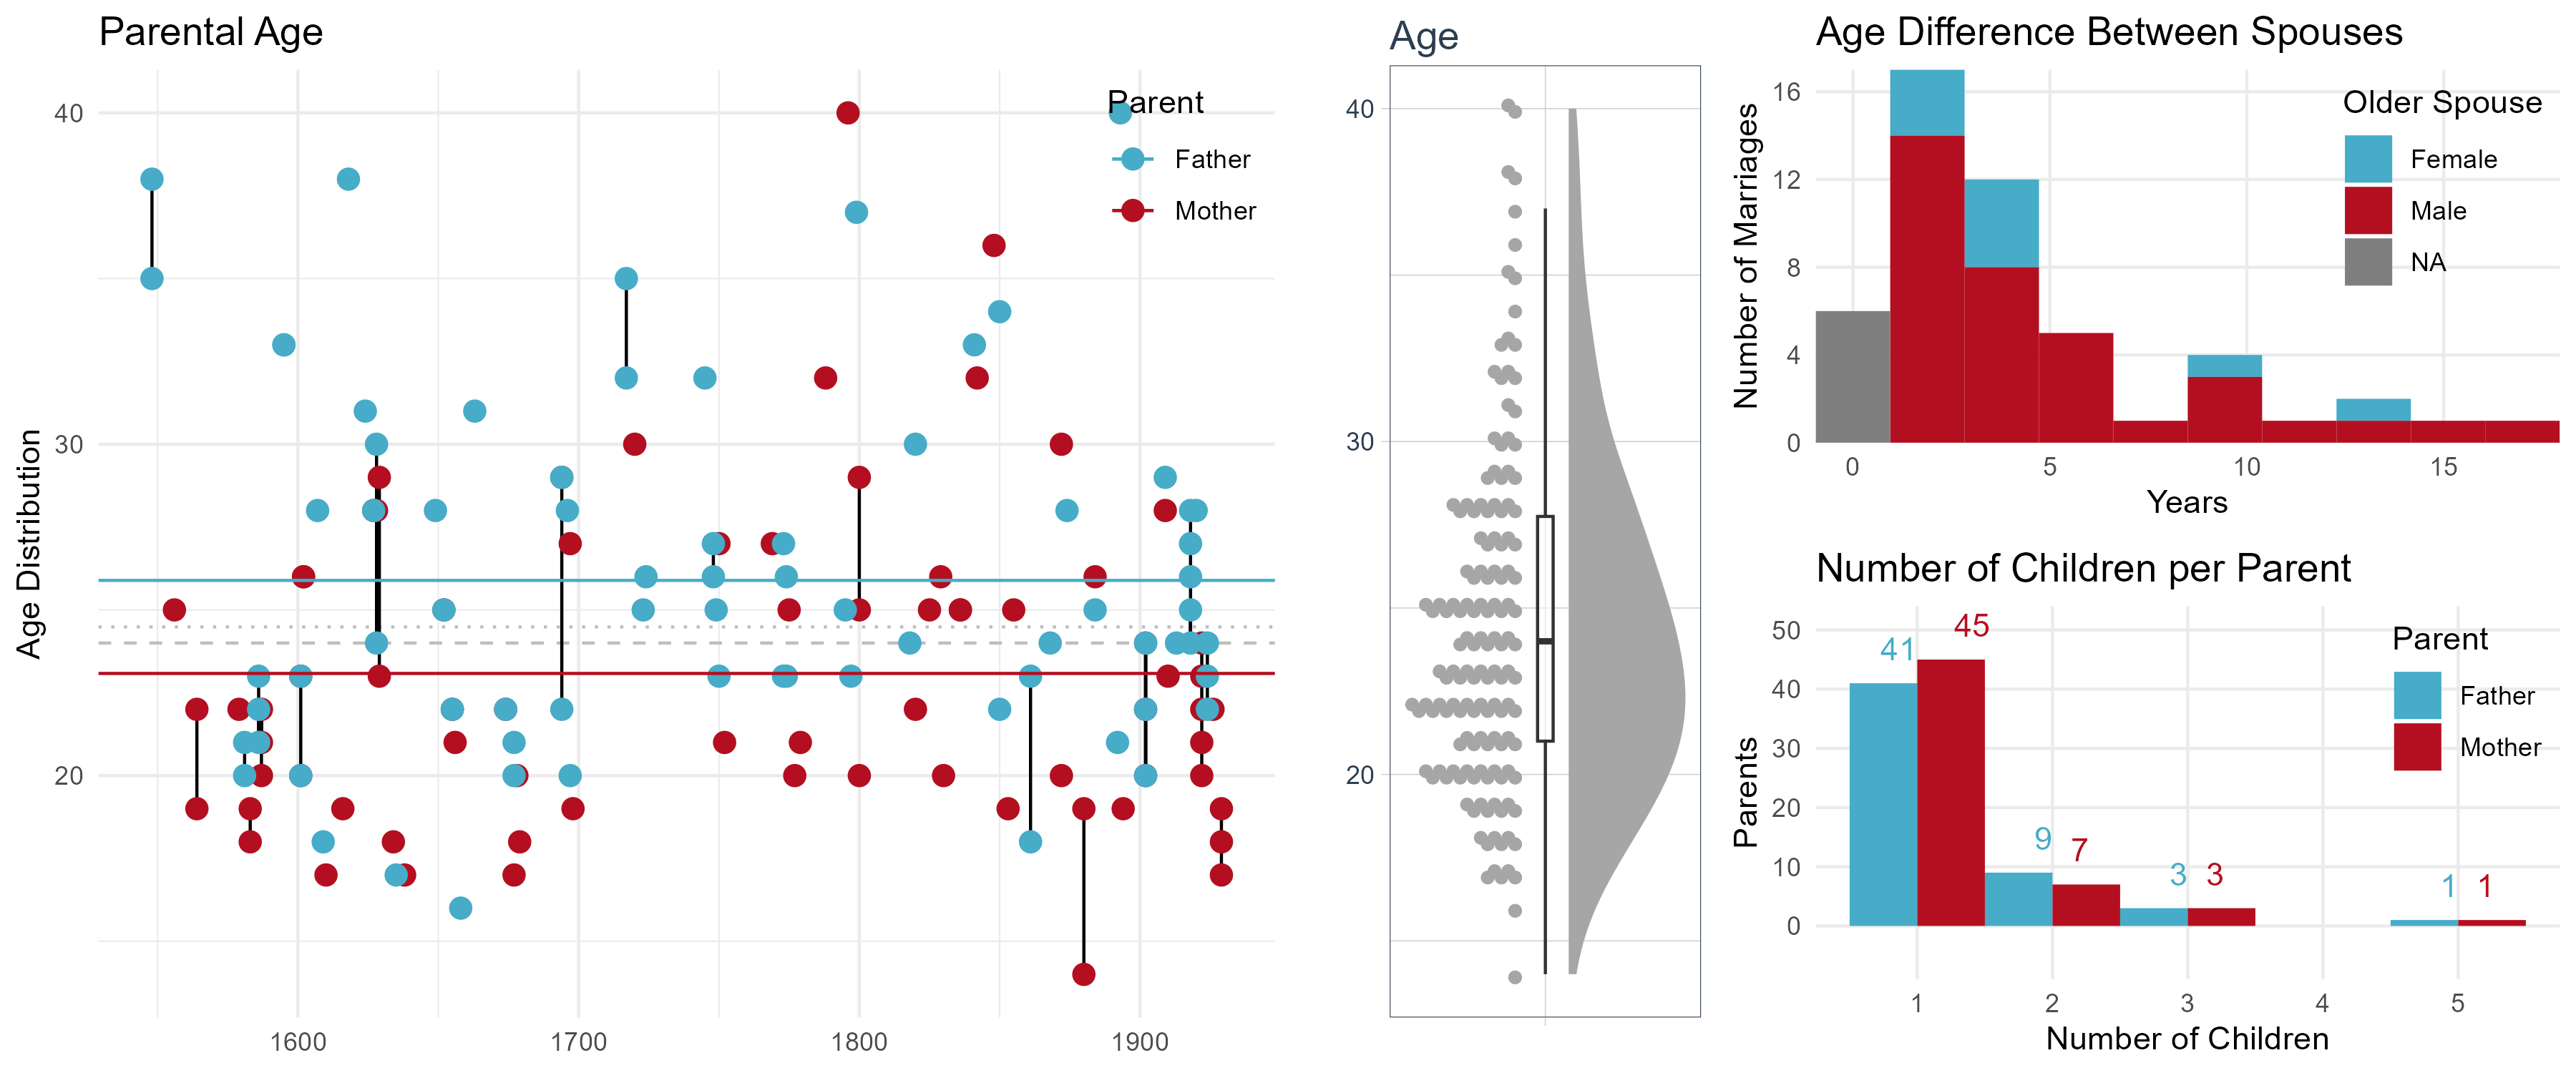
\includegraphics[width=\textwidth]{../rek-data-beers/R/figures/family_parent_age}
    \vspace{-18pt}
    \begin{itemize}
        \item 53 relationships described, 66 children born
        \item Average age of mother at childbirth is 23.5 years (fathers 26.0)
        \item 22 kids have either no father ($n=10$) or no mother ($n=12$)
        \item 85\% of marriages have an older husband, age difference generally 3 years (max 17 years)
    \end{itemize}
\end{frame}

\begin{frame}{Icelandic Naming Trends}
    \note{\tiny
    \begin{itemize}
    \item The 1980s saw \emph{Ísfólkið} evolve from mere literature to a defining cultural phenomenon.
    This saga resonated deeply. Real-world naming trends in Iceland began to mirror the saga's influence.
    \item For instance, names like \emph{Þula}, \emph{Yrja}, \emph{Heikir}, and especially \emph{Viljar}
    were virtually unheard of, only appearing in the Icelandic census after the series' publication.
    \item Our data highlights striking increases for several names post-publication of the saga.
    For example, the name \emph{Sunna} saw an almost 4-fold increase, \emph{Silja} doubled in its usage,
    and \emph{Saga} experienced a remarkable 5-fold surge.
    \item This being said, the data can sometimes be misleading. The surge in the use of the name \emph{Sölvi},
    for instance, is unlikely to be because of \emph{Ísfólkið}. The character of Sölvi in the saga, being malevolent,
    is hardly the type parents would choose as an inspiration. On the other hand, names like \emph{Heikir}, \emph{Yrja},
    and \emph{Viljar} were associated with beloved characters, making it understandable for parents to name their children after them.
    \item Yet, certain names, like \emph{Villimey}, remained unique to the saga, with no real-world adoptions even post-introduction.
    \item This data, generously provided by Yngvi Gautsson of \emph{Utopia Arctica},
    illuminates the saga's tangible influence while also rectifying some misconceptions from my initial Reykjavík DataBeer Talk.
    \end{itemize}
    The undeniable influence of \emph{Ísfólkið} on Icelandic naming trends underscores the profound cultural impact Margit's saga has had on our society.
}
    \centering
    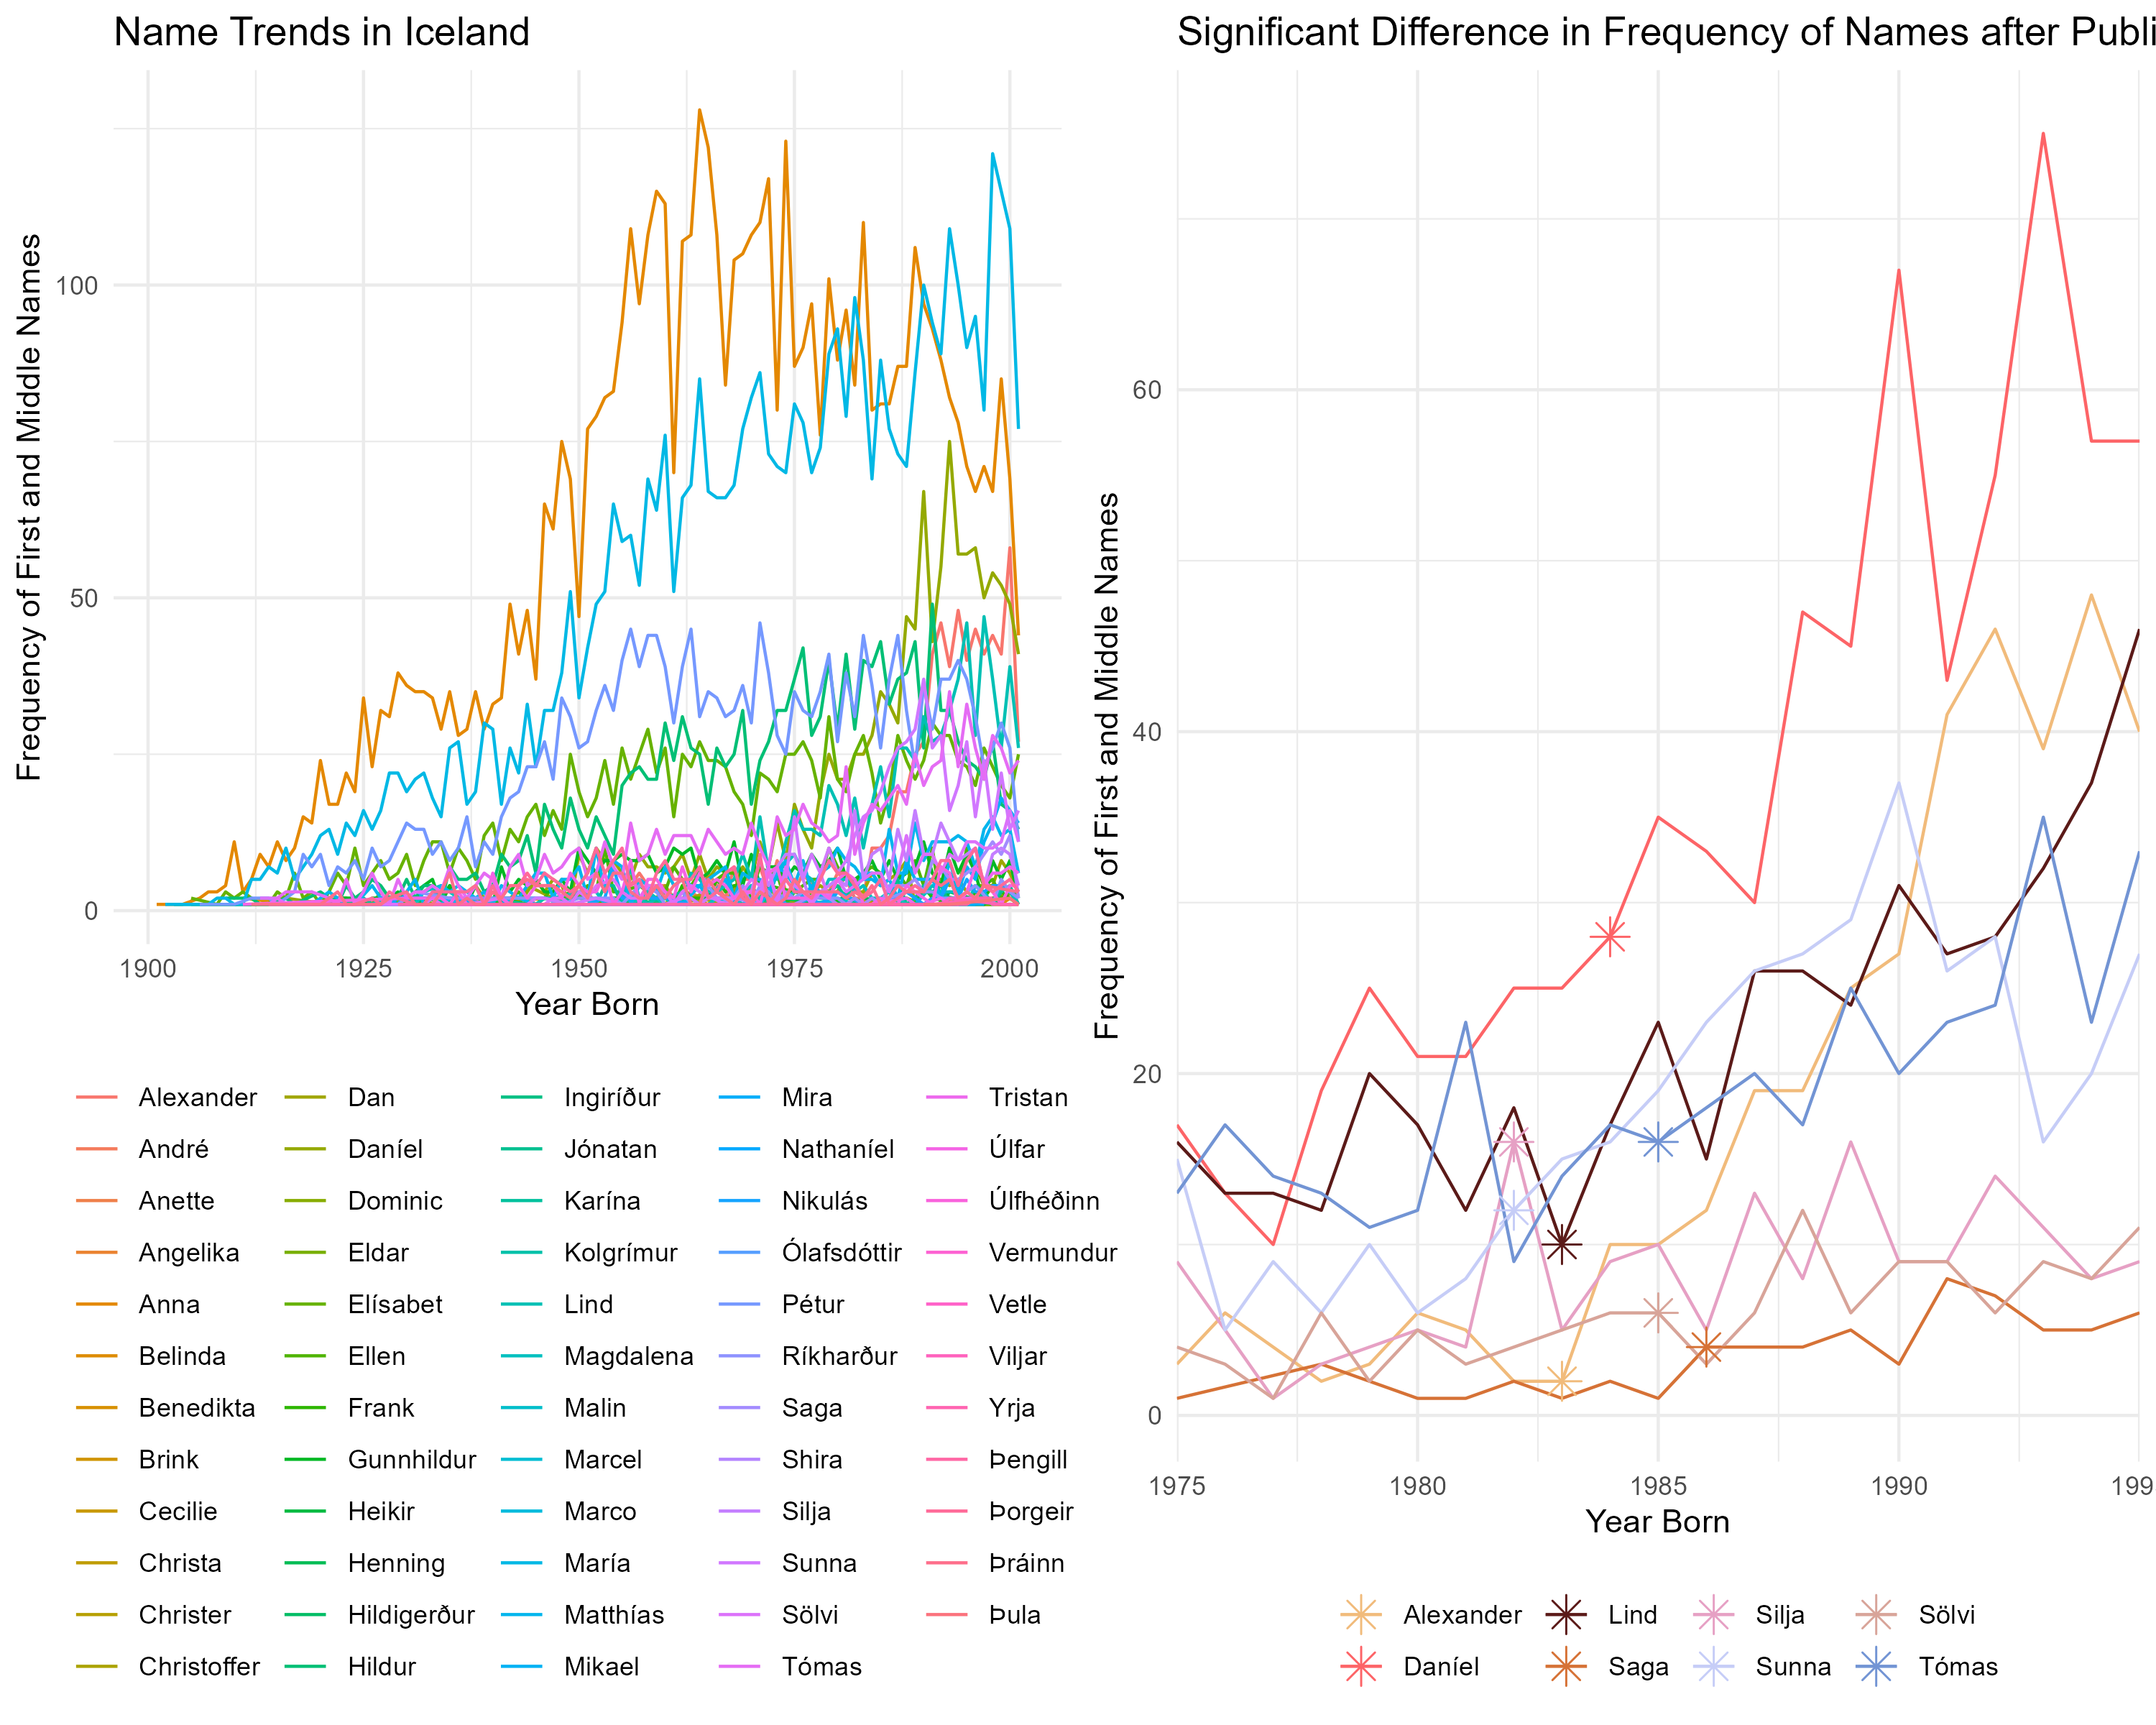
\includegraphics[width=\textwidth]{../rek-data-beers/R/figures/iceland_names.png}
    \vspace{-18pt}
    \begin{itemize}
        \item Protagonists' names \emph{Yrja}, \emph{Þula}, \emph{Heikir} and \emph{Viljar} first appear in the census
        a few years after Margit introduced them in her saga.
        \item Icelandic census data provided by Yngvi Gautsson of \emph{Utopia Arctica}
    \end{itemize}
\end{frame}
